\documentclass{article}
\usepackage{bm,sectsty,fancyhdr,multicol,lastpage}
\usepackage{amsmath,enumitem,tabularx,textcomp,nccmath,amssymb}
\usepackage{listings} % Insert bullet points
\usepackage[a4paper,left=1cm,right=1cm,top=2cm,bottom=2cm,headsep=0.5cm]{geometry}
\usepackage{xcolor} % Format color in code cells
\usepackage{titlesec} % Format title section
\usepackage{graphicx} % Embed images
\usepackage[document]{ragged2e} % Fix uneven spacing caused in multi col mode

% Define Colors
\definecolor{codegreen}{rgb}{0,0.6,0}
\definecolor{codegray}{rgb}{0.5,0.5,0.5}
\definecolor{codeorange}{rgb}{1,0.49,0}
\definecolor{backcolour}{rgb}{0.95,0.95,0.96}
\lstdefinestyle{mystyle}{
    backgroundcolor=\color{backcolour},
    commentstyle=\color{codegray},
    keywordstyle=\color{codeorange},
    numberstyle=\tiny\color{codegray},
    stringstyle=\color{codegreen},
    %basicstyle=\ttfamily\footnotesize,
    basicstyle=\tiny,
    breakatwhitespace=false,
    breaklines=true,
    captionpos=b,
    keepspaces=true,
    numbers=left,
    numbersep=5pt,
    showspaces=false,
    showstringspaces=false,
    showtabs=false,
    tabsize=2,
    xleftmargin=0pt,
    language=Python,
    label={lst:code},
    mathescape=true,
    gobble=20
}
\lstset{style=mystyle}


% Header and Footer
\pagestyle{fancy}
\fancyhf{}
\fancyhead[L]{CS Cheatsheet}
\fancyfoot[R]{Riten Patel}
\fancyfoot[L]{\LaTeX}
\fancyfoot[C]{\thepage\ of \pageref{LastPage}}
\renewcommand{\headrulewidth}{1.4pt}
\renewcommand{\footrulewidth}{1.4pt}

% Configurations
\sectionfont{\large}
\setlength{\columnsep}{0.5cm}
\setlength{\columnseprule}{1.4pt}
\setlength{\parindent}{0pt}
\setlength{\parskip}{-6pt}
\newcolumntype{Y}{>{\centering\arraybackslash}X}
\setlist[itemize]{nolistsep,left=0pt}
\graphicspath{{./images/}}
\tolerance=9999
\emergencystretch=10pt
\hyphenpenalty=10000
\exhyphenpenalty=100

\begin{document}
\begin{multicols*}{3}
    \raggedcolumns

    % Big O Notation
    \titleformat{\section}
        {\normalfont\fontfamily{phv}\fontsize{10}{0}\bfseries}{\thesection}{1em}{}
        \section{Big O Notation}
    \renewcommand\labelitemi{{\boldmath$\cdot$}}
    \setlist{nolistsep}
    \begin{itemize}[noitemsep]
        \item Asymptotic Notation - measures time and space complexity of an algorithm
        \begin{center}
            \begin{tabular}{||l l||}
                \hline
                Name & Magnitude  \\ [0.5ex]
                \hline\hline
                Constant & $O(1)$ \\
                \hline
                Logarithmic & $O(log n)$ \\
                \hline
                Linear & $O(n)$ \\
                \hline
                Superlinear & $O(n log n)$ \\
                \hline
                Polynomial & $O(n^{c})$ \\
                \hline
                Exponential & $O(c^{n})$ \\
                \hline
            \end{tabular}
        \end{center}
        \item Big O - upper bound (worst case)
        \item Big $\Omega$ - lower bound (best case)
        \item Big $\Theta$ - tight bound (avg case)
    \end{itemize}


    % Array Sequences
    \titleformat{\section}
        {\normalfont\fontfamily{phv}\fontsize{10}{0}\bfseries}{\thesection}{1em}{}
        \section{Array Sequences}
    \renewcommand\labelitemi{{\boldmath$\cdot$}}
    \begin{itemize}[noitemsep]
        \item Introduction
            \begin{itemize}[noitemsep]
                \item Byte is a memory address
                \item Byte = 8 bits
                \item Unicode char = 16 bits 
                \item Computer's main memory performs as random access memory (RAM). RAM allows any byte of main memory to be efficiently accessed.
            \end{itemize}
        \item Low Level Arrays 
            \begin{itemize}[noitemsep]
                \item Array - group of related variables stored in a contiguous portion of memory.
                \item Each cell uses the same number of bytes. Hence, any cell can be accessed in constant time.\\ 
                $value = start + (cellsize)(index)$
                \item Referential Array - each element refers to the object, 
                this way each element is still the same size. Multiple elements can refer 
                to the same object. An object can be shared by multiple lists.
                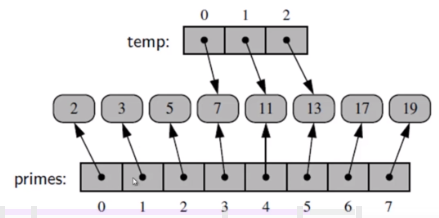
\includegraphics[width=\linewidth]{referential_array}
            \end{itemize}
        \item Dynamic Array
            \begin{itemize}[noitemsep]
                \item Don't need to specify how large an array is beforehand. 
                A list has greater capacity than current length. New array should have twice the capacity of the 
                existing array.
            \end{itemize}
    \end{itemize}


    % Stacks, Queues, Deques
    \titleformat{\section}
        {\normalfont\fontfamily{phv}\fontsize{10}{0}\bfseries}{\thesection}{1em}{}
    \section{Stacks, Queues, and Deques}
    \renewcommand\labelitemi{{\boldmath$\cdot$}}
    \begin{itemize}[noitemsep]
        \item Stack (LIFO, FILO)
        \begin{itemize}
            \item ordered collection of items where addition/removal of items
            takes place at the same end
            \item items closest to base have been there longest
            \item LIFO - (last-in, first-out) most recent items, removed first
            \item Applications: browser back button, back button pops out 
            webpages pushed onto stack
        \end{itemize}
        \item Queue (FIFO)
        \begin{itemize}
            \item ordered collection of items where addition/removal of items 
            takes place at opposite ends
            \item FIFO - (first-in, first-out) oldest item is removed first
            \item Enqueue - add a new to queue
            \item Dequeue - remove front item of queue
            \item Applications: movie ticket line, grocery line, \dots
        \end{itemize}
        \item Deque
        \begin{itemize}
            \item ordered collection of items with two ends 
            \item new items added/removed at both ends
        \end{itemize}
    \end{itemize}


    % Linked Lists
    \titleformat{\section}
        {\normalfont\fontfamily{phv}\fontsize{10}{0}\bfseries}{\thesection}{1em}{}
    \section{Linked Lists}
    \renewcommand\labelitemi{{\boldmath$\cdot$}}
    \begin{itemize}[noitemsep]
        \item Singly Linked Lists
        \begin{itemize}
            \item Collection of nodes that form a linear sequence.
            \item Each node stores a reference to an object that is 
            an element of the sequence and a reference to the next node of the list.
            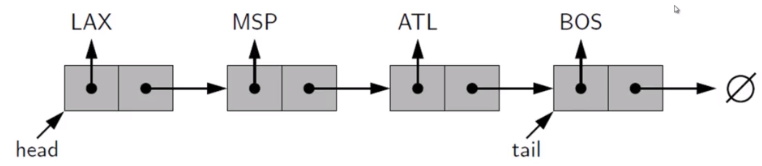
\includegraphics[width=\linewidth]{singly_linked_list}                
            \item No predetermined fixed size
            \item Pros: insertions/deletions $O(1)$
            \item Cons: access/search takes $O(n)$
        \end{itemize}
        \item Doubly Linked Lists 
        \begin{itemize}
            \item linked list in which each node keeps a reference
            to the node before/after it
            \item sentinel - header/trailer nodes
            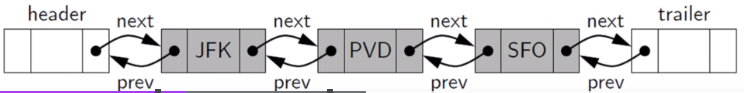
\includegraphics[width=\linewidth]{doubly_linked_list}
            \item inserting a node between two nodes is easy
            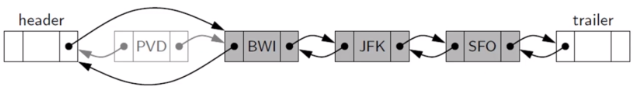
\includegraphics[width=\linewidth]{doubly_linked_list_insertion}
        \end{itemize}
    \end{itemize}


    % Recursion
    \titleformat{\section}
        {\normalfont\fontfamily{phv}\fontsize{10}{0}\bfseries}{\thesection}{1em}{}
    \section{Recursion}
    \renewcommand\labelitemi{{\boldmath$\cdot$}}
    \begin{itemize}[noitemsep]
        \item Two types
        \begin{itemize}
            \item Function that calls itself
            \item Data structure represented with same data structures
            \item Always start with the base case
        \end{itemize}
        \item Memoization
        \begin{itemize}
            \item Remembering result of method calls by inputs and returning
            cached results rather than re-computing.
        \end{itemize}
    \end{itemize}


    % Trees
    \titleformat{\section}
        {\normalfont\fontfamily{phv}\fontsize{10}{0}\bfseries}{\thesection}{1em}{}
    \section{Trees}
    \renewcommand\labelitemi{{\boldmath$\cdot$}}
    \begin{itemize}[noitemsep]
        \item What is a Tree?
        \begin{itemize}
            \item Has roots, branches, and leaves
            \item Ex: animal kingdom, file system, html, ...
            \item Node - has a key (name) and payload (attributes)
            \item Edge - connects two nodes to form a relationship. The root node is 
            the only one with no incoming edges.
            \item Path - ordered list of nodes connected by edges
            \item Children - nodes that have incoming edges from the same node.
            \item Parent - node with outgoing edges to children
            \item Leaf - node with no children
            \item Level - num of edges on path from root node to $n$
            \item Trees - set of nodes and edges connected to each other. \\
            (1) One node is designated as root node, 
            (2) every node except root is connected by at least one other node,
            (3) a unique path traverses from root to each node
            (4) binary tree - each node has max of two children
            \item Recursive Definition - tree is empty or consists of nested subtrees
        \end{itemize}
        \item Implement Trees as List of Lists
        \begin{itemize}
            \item Store as [root, left subtree, right subtree]
            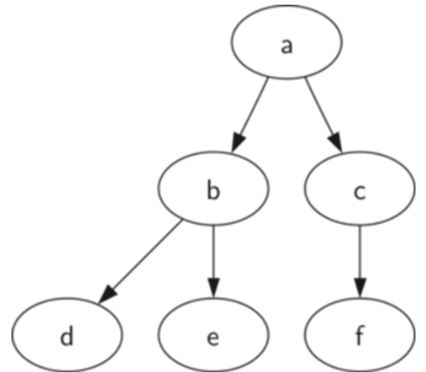
\includegraphics[width=\linewidth]{trees_implementation}
            \begin{lstlisting}
                    myTree = ['a', #root
                                ['b', #left subtree
                                    ['d',[],[]],
                                    ['e',[],[]] ],
                                ['c', #right subtree
                                    ['f',[],[]] ]
                             ] 
            \end{lstlisting}
        \end{itemize}
        \item Tree Traversals \\
        3 patterns to visit all nodes in a tree
        \begin{itemize}
            \item Preorder: root, left preorder, right preorder
            \item Inorder: left inorder, root, right inorder
            \item Postorder: left postorder, right postorder, root
            \item Remember "post/in/pre" refers to the placement of processing the root node
            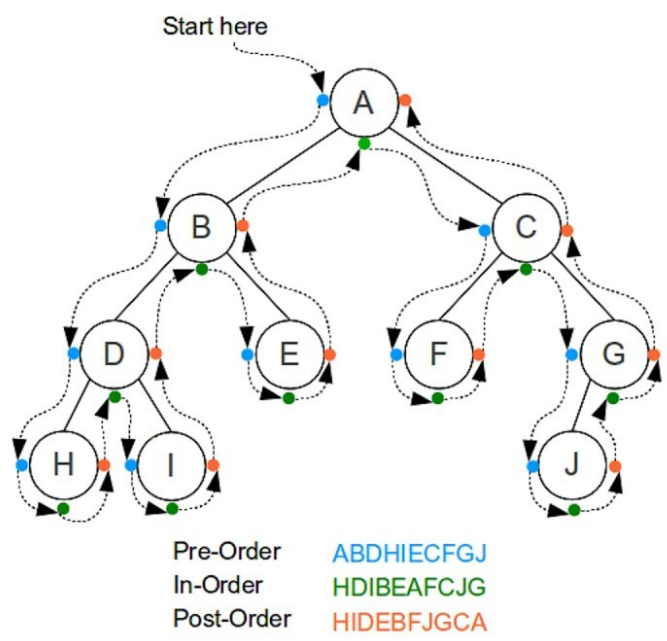
\includegraphics[width=\linewidth]{pre_in_post_order} \\
        \end{itemize}
        \item Priority Queues with Binary Heaps
        \begin{itemize}
            \item Like a queue(i.e. FIFO) but order of items is determined by 
            their priority
            \item Highest at front, lowest at back
            \item Binary Heap - $O(log n)$ \\
            1. Create a Complete Binary Tree - Balanced Tree \\
            2. Order heap from smallest to largest  \\
            3. If p = index of parent, \\ 
               index of children = (2p,2p+1)
        \end{itemize}
        \item Binary Search Tree (BST)
        \begin{itemize}
            \item 2 implementations of map ADT \\
            1. Binary Search on list \\
            2. Hash Tables \\
            \item Three properties \\
            1. left subtree of a node contains only nodes with keys less than node's key \\
            2. right subtree of a node contains only nodes with keys greater than node's key \\
            3. left and right subtree each must also be a binary search tree \\
            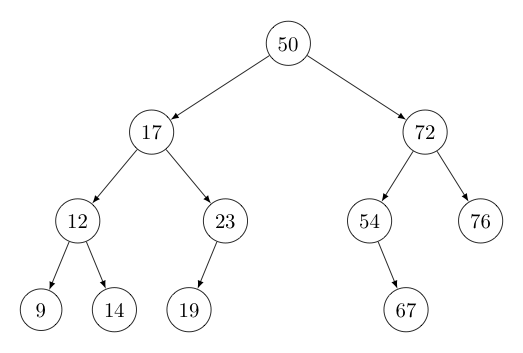
\includegraphics[width=\linewidth]{binary_search_tree}
        \end{itemize}
        \item B-Tree
        \begin{itemize}
            \item a self-balanced tree in which every node has multiple keys 
            and has more than two children
            \item search/insertion is similar to BSTs \\
            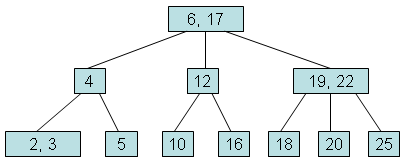
\includegraphics[width=\linewidth]{b-tree2}
        \end{itemize}
    \end{itemize}


    % Searching and Sorting
    \titleformat{\section}
        {\normalfont\fontfamily{phv}\fontsize{10}{0}\bfseries}{\thesection}{1em}{}
    \section{Searching and Sorting}
    \renewcommand\labelitemi{{\boldmath$\cdot$}}
    \begin{itemize}[noitemsep]
    \item Sequential Search
    \item Binary Search \\
        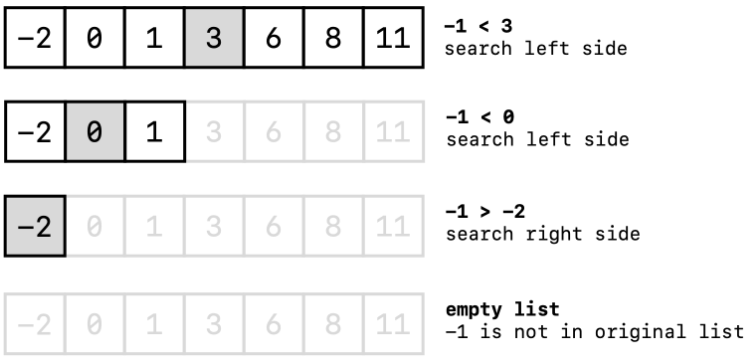
\includegraphics[width=\linewidth]{binary_search} \\
        \begin{itemize}
            \item Divide and Conquer - divide problem
            into smaller pieces, reassemble to get result \\
            iter 1, array length = $n$ \\
            iter 2, array length = $n/2$ \\
            iter 3, array length = $n/2 * (1/2)$ \\
            after iter i, array length = $n/2^i$ \\
            \textbf{after i iter, array length = 1} \\
            $1 = n/2^i$ \\
            $2^i = n$ \\
            $ilog(2) = log(n)$ \\
            $i = log(n)$
        \end{itemize}
    \item Hashing
        \begin{itemize}
            \item hash table - collection of items stored
            in a way to make it easy to find later
            \item hash function - mapping between item 
            and slot where item belongs
            \item perfect hash function - maps each item into 
            a unique slot
            \item load factor: tradeoff between time and space: \\
            $\lambda = num items/tablesize$ \\
            $\lambda = .75$ is a good rule of thumb
            \item To search use hash function to 
            lookup slot number and check
            \item $O(1)$
        \end{itemize}
    \item Hash Functions
        \begin{itemize}
            \item Remainder \\
            $h(item)=item\,\%\,len(table)$
            \item Folding \\
            1. Divide into equal-size pieces \\
            2. Add each piece \\
            3. Find remainder \\
            i.e. 436-555-4601 \\
            (43,65,55,46,01) \\
            43+65+55+46+01 = 210 \\
            210 \% 11 = 1
            \item Mid-Square \\
            1. Square item \\
            2. Extract middle $r$ digits \\
            3. Find remainder
            \item For strings \\
            1. Lookup ordinal value \\
            2. Add them up \\
            3. Find remainder
        \end{itemize}
    \item Collision Resolution
        \begin{itemize}
            \item linear probing - move sequentially and 
            reassign collision item to first empty slot
            \item chaining - items chained in same location
            \item searching is difficult with either
            resolution technique
        \end{itemize}
    \item Sorting
        \begin{itemize}
            \item Visualization Resources \\
            - www.sorting-algorithms.com \\
            - visualgo.net/sorting.html \\
            - en.wikipedia.org/wiki/
            \item Bubble sort \\
            - multiple passes through list \\
            - multiple exchanges per pass \\
            - compares adjacent items \\
            - largest bubbles to its place
            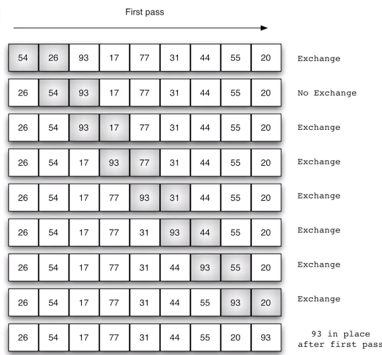
\includegraphics[width=\linewidth]{bubble_sort}
            \item Selection sort \\
            - one exchange per pass \\
            - puts largest into proper place
            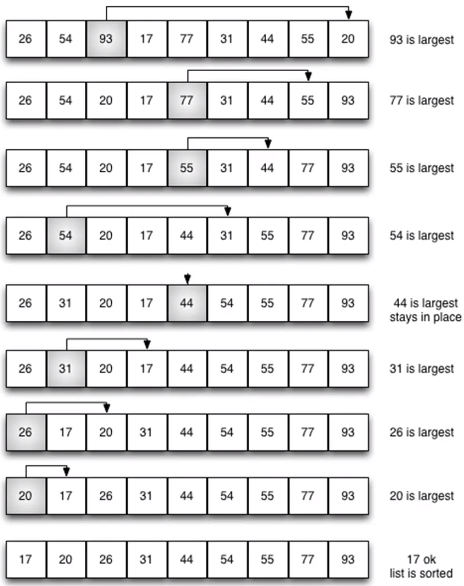
\includegraphics[width=\linewidth]{selection_sort}
            \item Insertion sort \\
            - check item with sorted sublist \\
            - shift items greater to the right \\
            - insert item when can't shift
            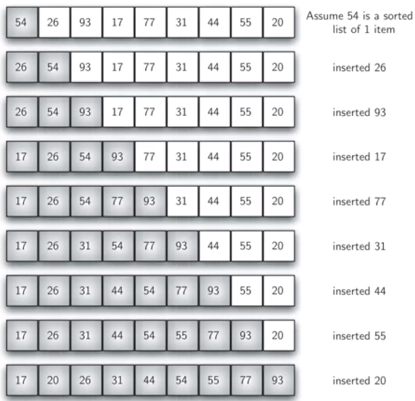
\includegraphics[width=\linewidth]{insertion_sort_part1}
            - how does insertion look like? \\
            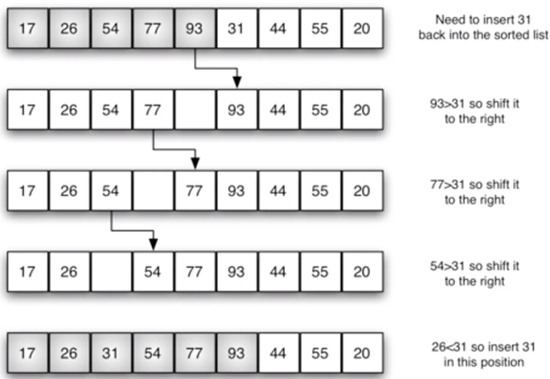
\includegraphics[width=\linewidth]{insertion_sort_part2}
            \item Shell sort \\
            - like insertion sort but with more sublists \\
            - perform earlier sublist sorts \\
            - reduces number of shifting operations \\
            - i.e. sublist increment of 3 \\
            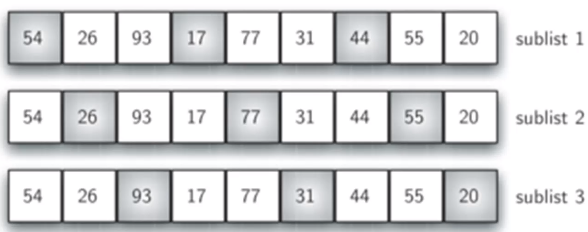
\includegraphics[width=\linewidth]{shell_sort_part1}
            - i.e. insertion sort sublists and combine \\
            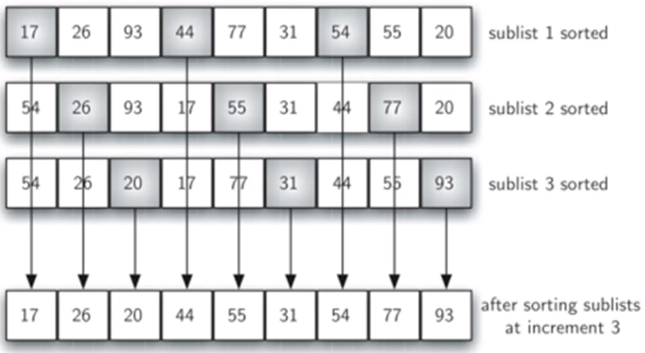
\includegraphics[width=\linewidth]{shell_sort_part2}
            - i.e. insertion sort final list \\
            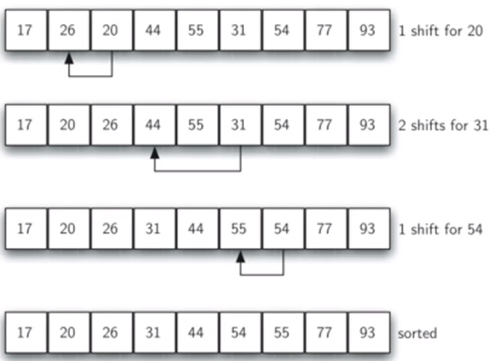
\includegraphics[width=\linewidth]{shell_sort_part3}
            \item Merge sort \\
            - divide and conquer algorithm \\
            - recursive splitting list in half \\
            - sort each split \\
            - merge back together \\
            - i.e. recursive splitting \\
            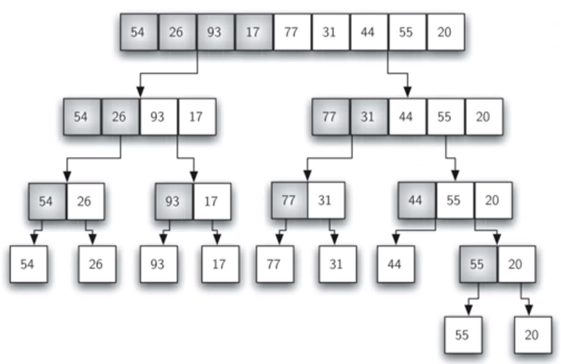
\includegraphics[width=\linewidth]{merge_sort_splitting}
            - i.e. merge and sort \\
            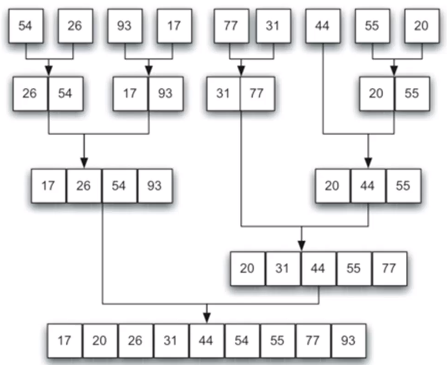
\includegraphics[width=\linewidth]{merge_sort_merging}
            \item Quick sort \\
            - divide and conquer algorithm \\
            - but doesn't use additional storage \\
            - however list may not be divided in half \\
            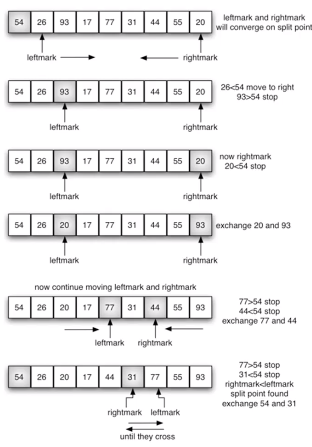
\includegraphics[width=\linewidth]{quick_sort_algorithm}
            \begin{center}
                %\begin{tabular}{||l l l||}
                \resizebox{\linewidth}{!}{%
                \begin{tabular}{lll}
                    \hline
                    Name & Worst & Best  \\ [0.5ex]
                    \hline\hline
                    Bubble Sort & $O(n^2)$ & $\Omega(n)$ \\
                    \hline
                    Selection Sort & $O(n^2)$ & $\Omega(n^2)$ \\
                    \hline
                    Insertion Sort & $O(n^2)$ & $\Omega(n)$ \\
                    \hline
                    Shell Sort & $O(n*(log(n))^2)$ & $\Omega(n*log(n))$ \\
                    \hline
                    Merge Sort & $O(n*log(n))$ & $\Omega(n*log(n))$ \\
                    \hline
                    Quick Sort & $O(n^2)$ & $\Omega(n*log(n))$ \\
                    \hline
                \end{tabular}}
            \end{center}
        \end{itemize}
    \end{itemize}


    % Graphs
    \titleformat{\section}
        {\normalfont\fontfamily{phv}\fontsize{10}{0}\bfseries}{\thesection}{1em}{}
    \section{Graphs}
    \renewcommand\labelitemi{{\boldmath$\cdot$}}
    \begin{itemize}[noitemsep]
        \item Graphs have nodes(vertices), edges that connect the nodes, 
        and optionally weights to show there is a cost to go from one vertex 
        to another
        \item $G = (V,E)$ where w,v$\in$V
        \item A path is a sequence of vertices connected by edges
        \item They are represented in three ways: 
        (from left to right: graph, adjacency matrix, adjacency list)
        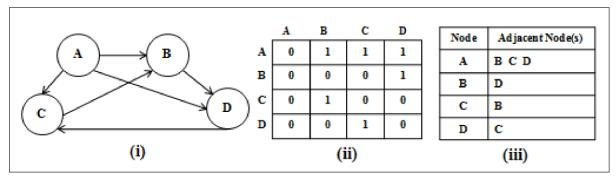
\includegraphics[width=\linewidth]{graphs_representation}
        \item Adjacency matrix is more time efficient.
        The adjacency matrix is simple and a good implementation 
        when the number of edges is large. It is mostly empty (i.e. sparse). 
        \item An adjacency list is more space efficient and allows us to compactly
        represent a sparse graph
        \item A cycle in a directed graph (digraph) is a path that starts/ends at the 
        same vertex
        \item Breadth First Search (BFS)
        \begin{itemize}
            \item Builds a search tree one level at a time
            \item Great explanation: https://www.youtube.com/watch?v=s-CYnVz-uh4
            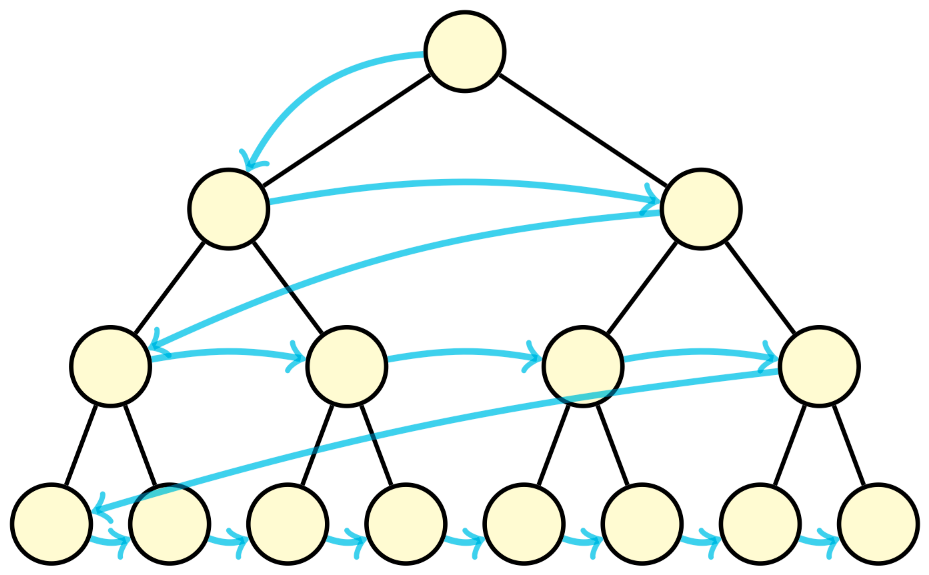
\includegraphics[width=\linewidth]{bfs_traversal}
            \item Application: Word Ladder Problem
            \begin{itemize}
                \item Transorm the word "FOOL" into the word "SAGE". You can only change
                one letter at a time. At each step, you must transform one word into 
                another word. You cannot transform a word into a non-word
                \item Solution: Use BFS to find an efficient
                path from starting to ending word. Get a list of all four letter words. 
                Replace one of the letters with an underscore and move words that match 
                the pattern into the appropriate bucket.
                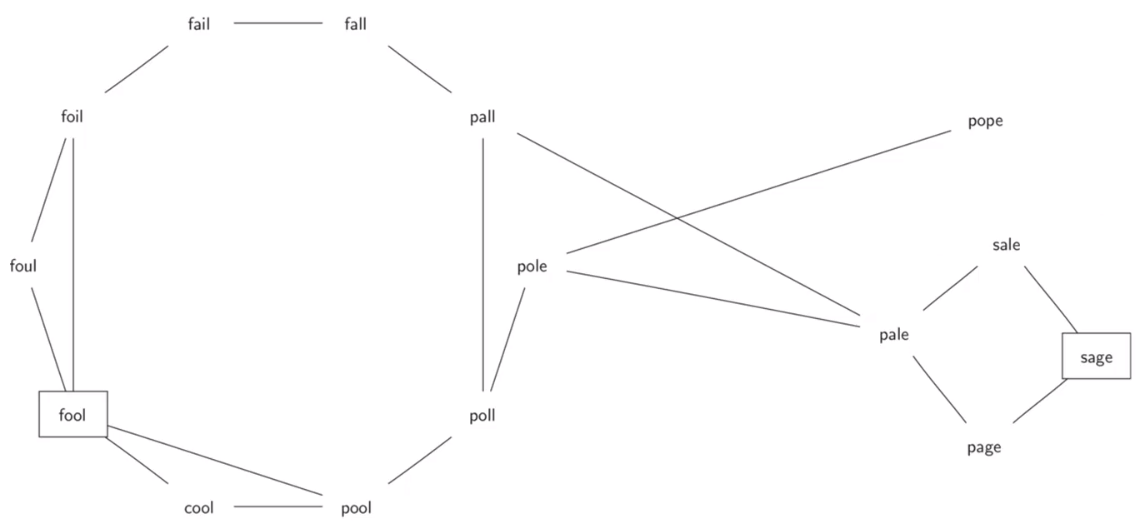
\includegraphics[width=\linewidth]{word_problem}
            \end{itemize}
        \end{itemize}
        \item Depth First Search (DFS)
        \begin{itemize}
            \item DFS builds a search tree by exploring one branch 
            of a tree as deeply as possible. 
            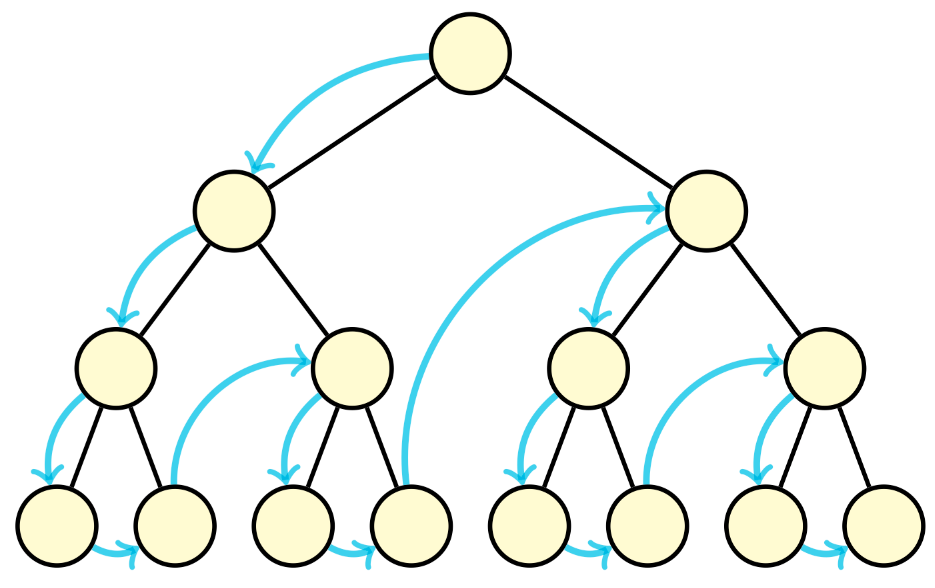
\includegraphics[width=\linewidth]{dfs_traversal}
            \item Knight's Tour Example Problem
            \begin{itemize}
                \item Suppose you have a chess board with a single chess piece, the knight.
                Find a sequence of moves that allows the knight to visit every square on 
                the board exactly once.
                \item Solution: Represent the moves of a knight on a chessboard as a graph. 
                Use DFS to find a path of length rows x columns - 1
                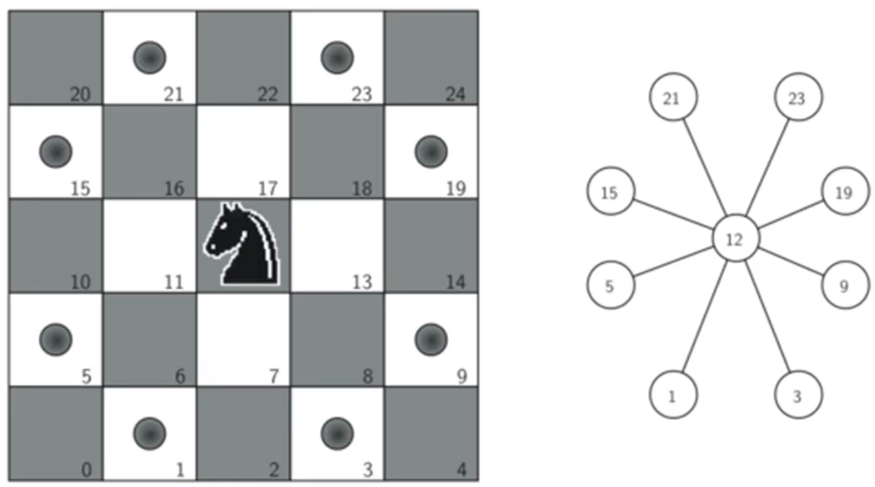
\includegraphics[width=\linewidth]{knights_problem_board}  \\
            \end{itemize}
        \end{itemize}
        \item Use BFS over DFS when \dots 
        \begin{itemize}
            \item the solution is not far from the root
            \item the tree is very deep and solutions are rare 
        \end{itemize}
        \item Use DFS over BFS when \dots 
        \begin{itemize}
            \item the tree is very wide. BFS might need too much memory
            \item solutions are frequent but located deep in the tree 
        \end{itemize}
    \end{itemize}
\end{multicols*}
    

    % Appendix
    \titleformat{\section}
        {\normalfont\fontfamily{phv}\fontsize{10}{0}\bfseries}{\thesection}{1em}{}
    \section{Appendix}
    \renewcommand\labelitemi{{\boldmath$\cdot$}}
    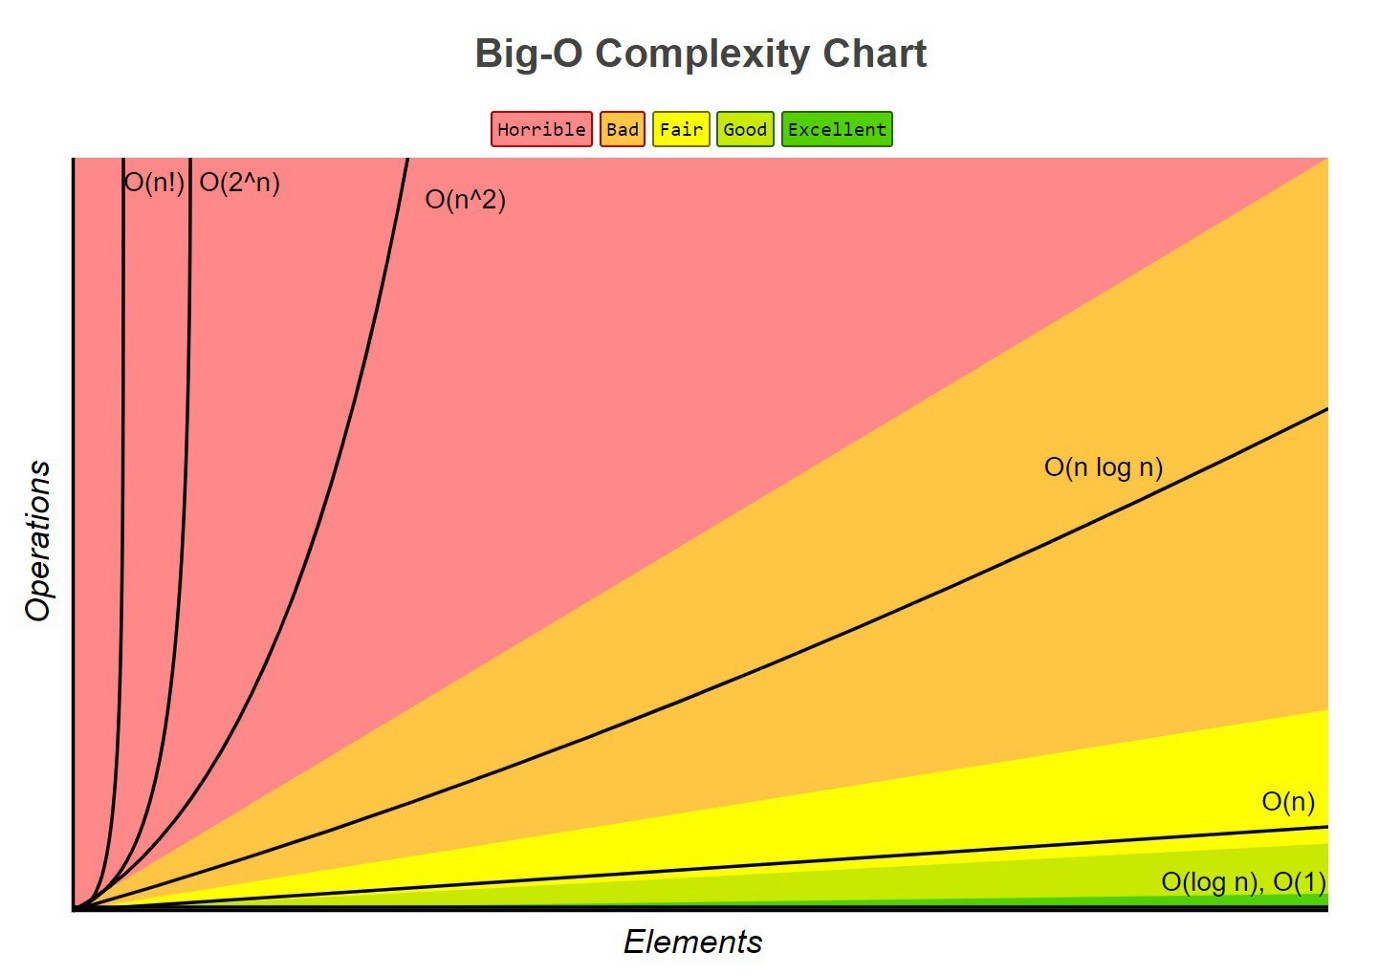
\includegraphics[width=\linewidth]{big_o_complexity_chart}
    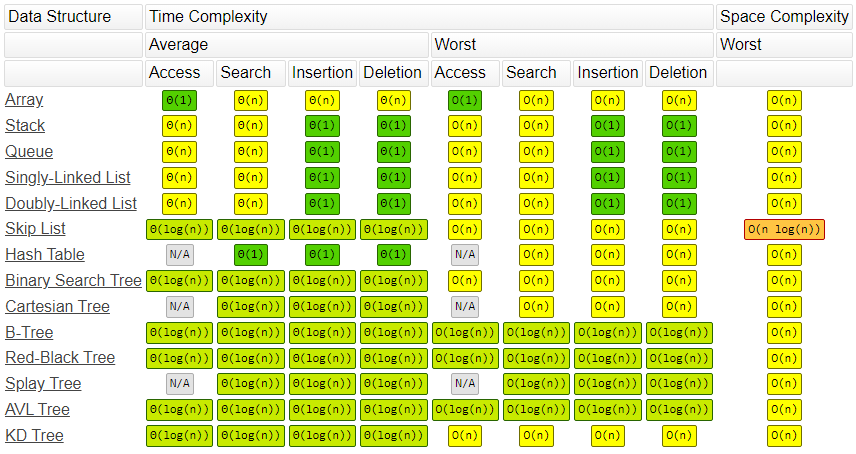
\includegraphics[width=\linewidth]{data_structures_big_o}
\end{document}
